% !TeX root = ../../../../thesis.tex


\subsection{Modulator}	
\label{subsec:ac-modulator}

The job of the modulator in an AC environment, is the same as in a DC environment.
Just like in the DC environment, when a `0' has to be encoded the current should be zero and when a `1' has to be encoded the current should be some constant value.
The transition between a `0' and `1' should be fast, so that a square wave is created, just like in the DC case.

If the translation is done in this manner, the mapping between the code sequence symbols and the current is clear and the aggregated current drawn by multiple lights will also be a square wave, which will allow for decoding the information.
Next, existing hardware is investigated to see if they can modulate the current draw as ideal square waves.
%if these solutions will translate the IDs into a current draw which is similar to what has just been discussed above. 



% !TeX root = ../../../../../thesis.tex


\subsubsection{SMPS and LED}

In \autoref{fig:ac-smps-led-and-smps-picture} a commercial LED lighting fixture can be seen with a switching mode power supply (SMPS).
The power supply transforms the AC to a DC signal which is used to power the LED.




For this setup it is investigated what the current signature looks like when the LED is on, representing a `1', and when the LED is off,  representing a `0'.
A 10 ohm resistor is placed in series with the SMPS on the AC side and the voltage drop over this resistor is measured.
So a voltage is measured, but the current that flows can be calculated using Ohm's law: $I = \frac{U}{R}$.
But since we are investigating how the current signature behaves, it is not needed to have exact numbers on the current draw.








\begin{figure}[h]
	\centering     %%% not \center
	\subfigure[Encoding a `0', LED off.]{
		\label{fig:smps-current-primary-no-load}
		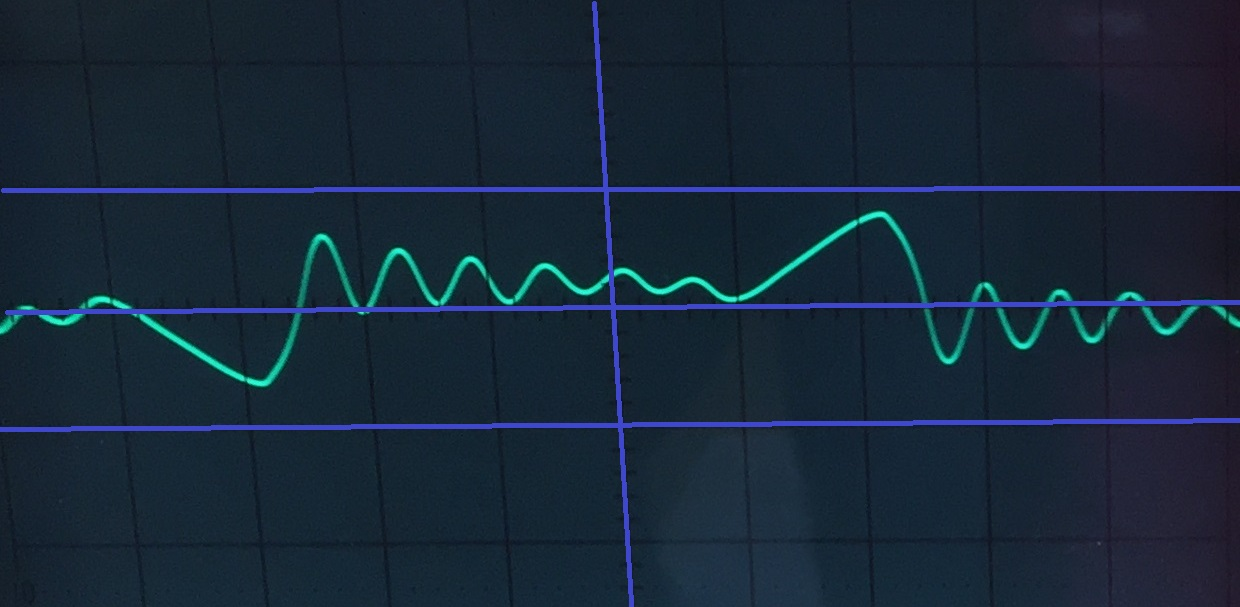
\includegraphics[width=60mm]
		{chapters/hardware-chapters/AC/ac-modulator/smps-led/smps-current-primary-no-load-cropped-edit.jpg}
	}
	\subfigure[Encoding a `1', LED on.]{ 
		% 33 ohm...
		\label{fig:smps-current-primary-with-load}
		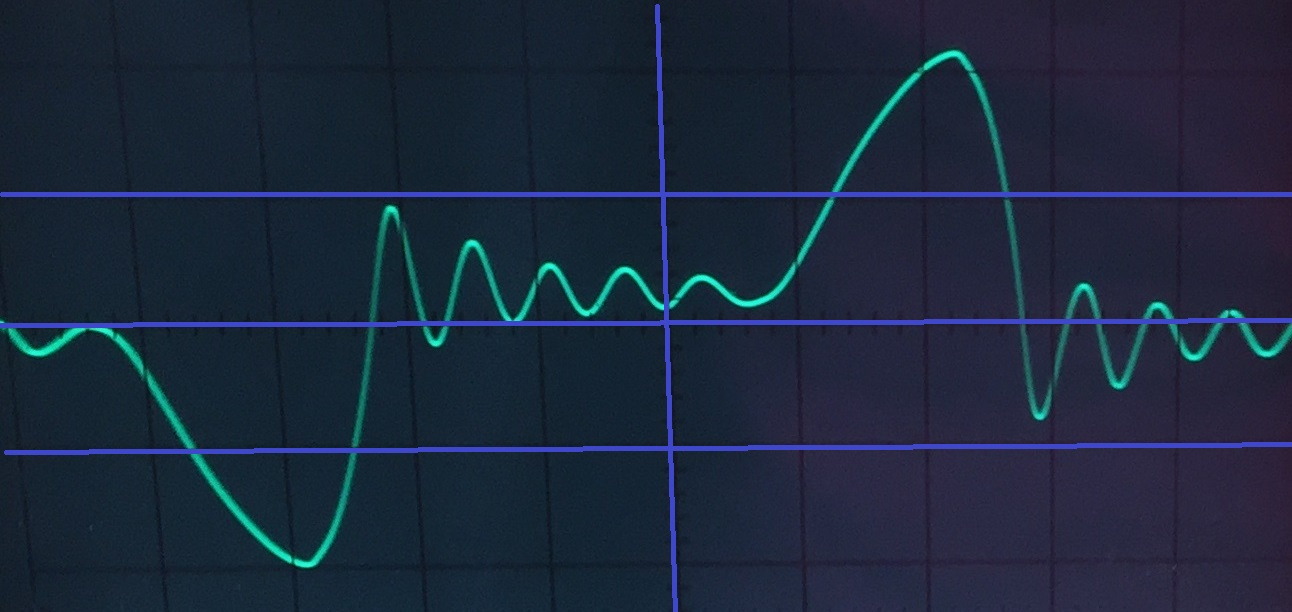
\includegraphics[width=60mm]
		{chapters/hardware-chapters/AC/ac-modulator/smps-led/smps-current-primary-with-load-cropped-edit.jpg}
	}

	\caption{Voltage measured over a 10 ohm series resistor at the primary side, to determine the current flow in two situations of a SMPS, when encoding a `0' and a `1'. X-axis: 2 ms/div, Y-axis: 500 mV/div.}
\end{figure}






In Figures \ref{fig:smps-current-primary-no-load} and \ref{fig:smps-current-primary-with-load} the current signature of the SMPS can be seen, when encoding a `0' (LED off) and when encoding a `1' (LED on), respectively.
From these figures, it is clear to see that when encoding a zero, the current is not zero and when encoding a `1', the current is not a constant value.
This makes it difficult to determine what the ID is of this transmitting LED.
This becomes even more difficult when multiple of these current signatures will be superimposed.








	\begin{figure}
		\centering
		\begin{minipage}[b]{0.45\textwidth}
			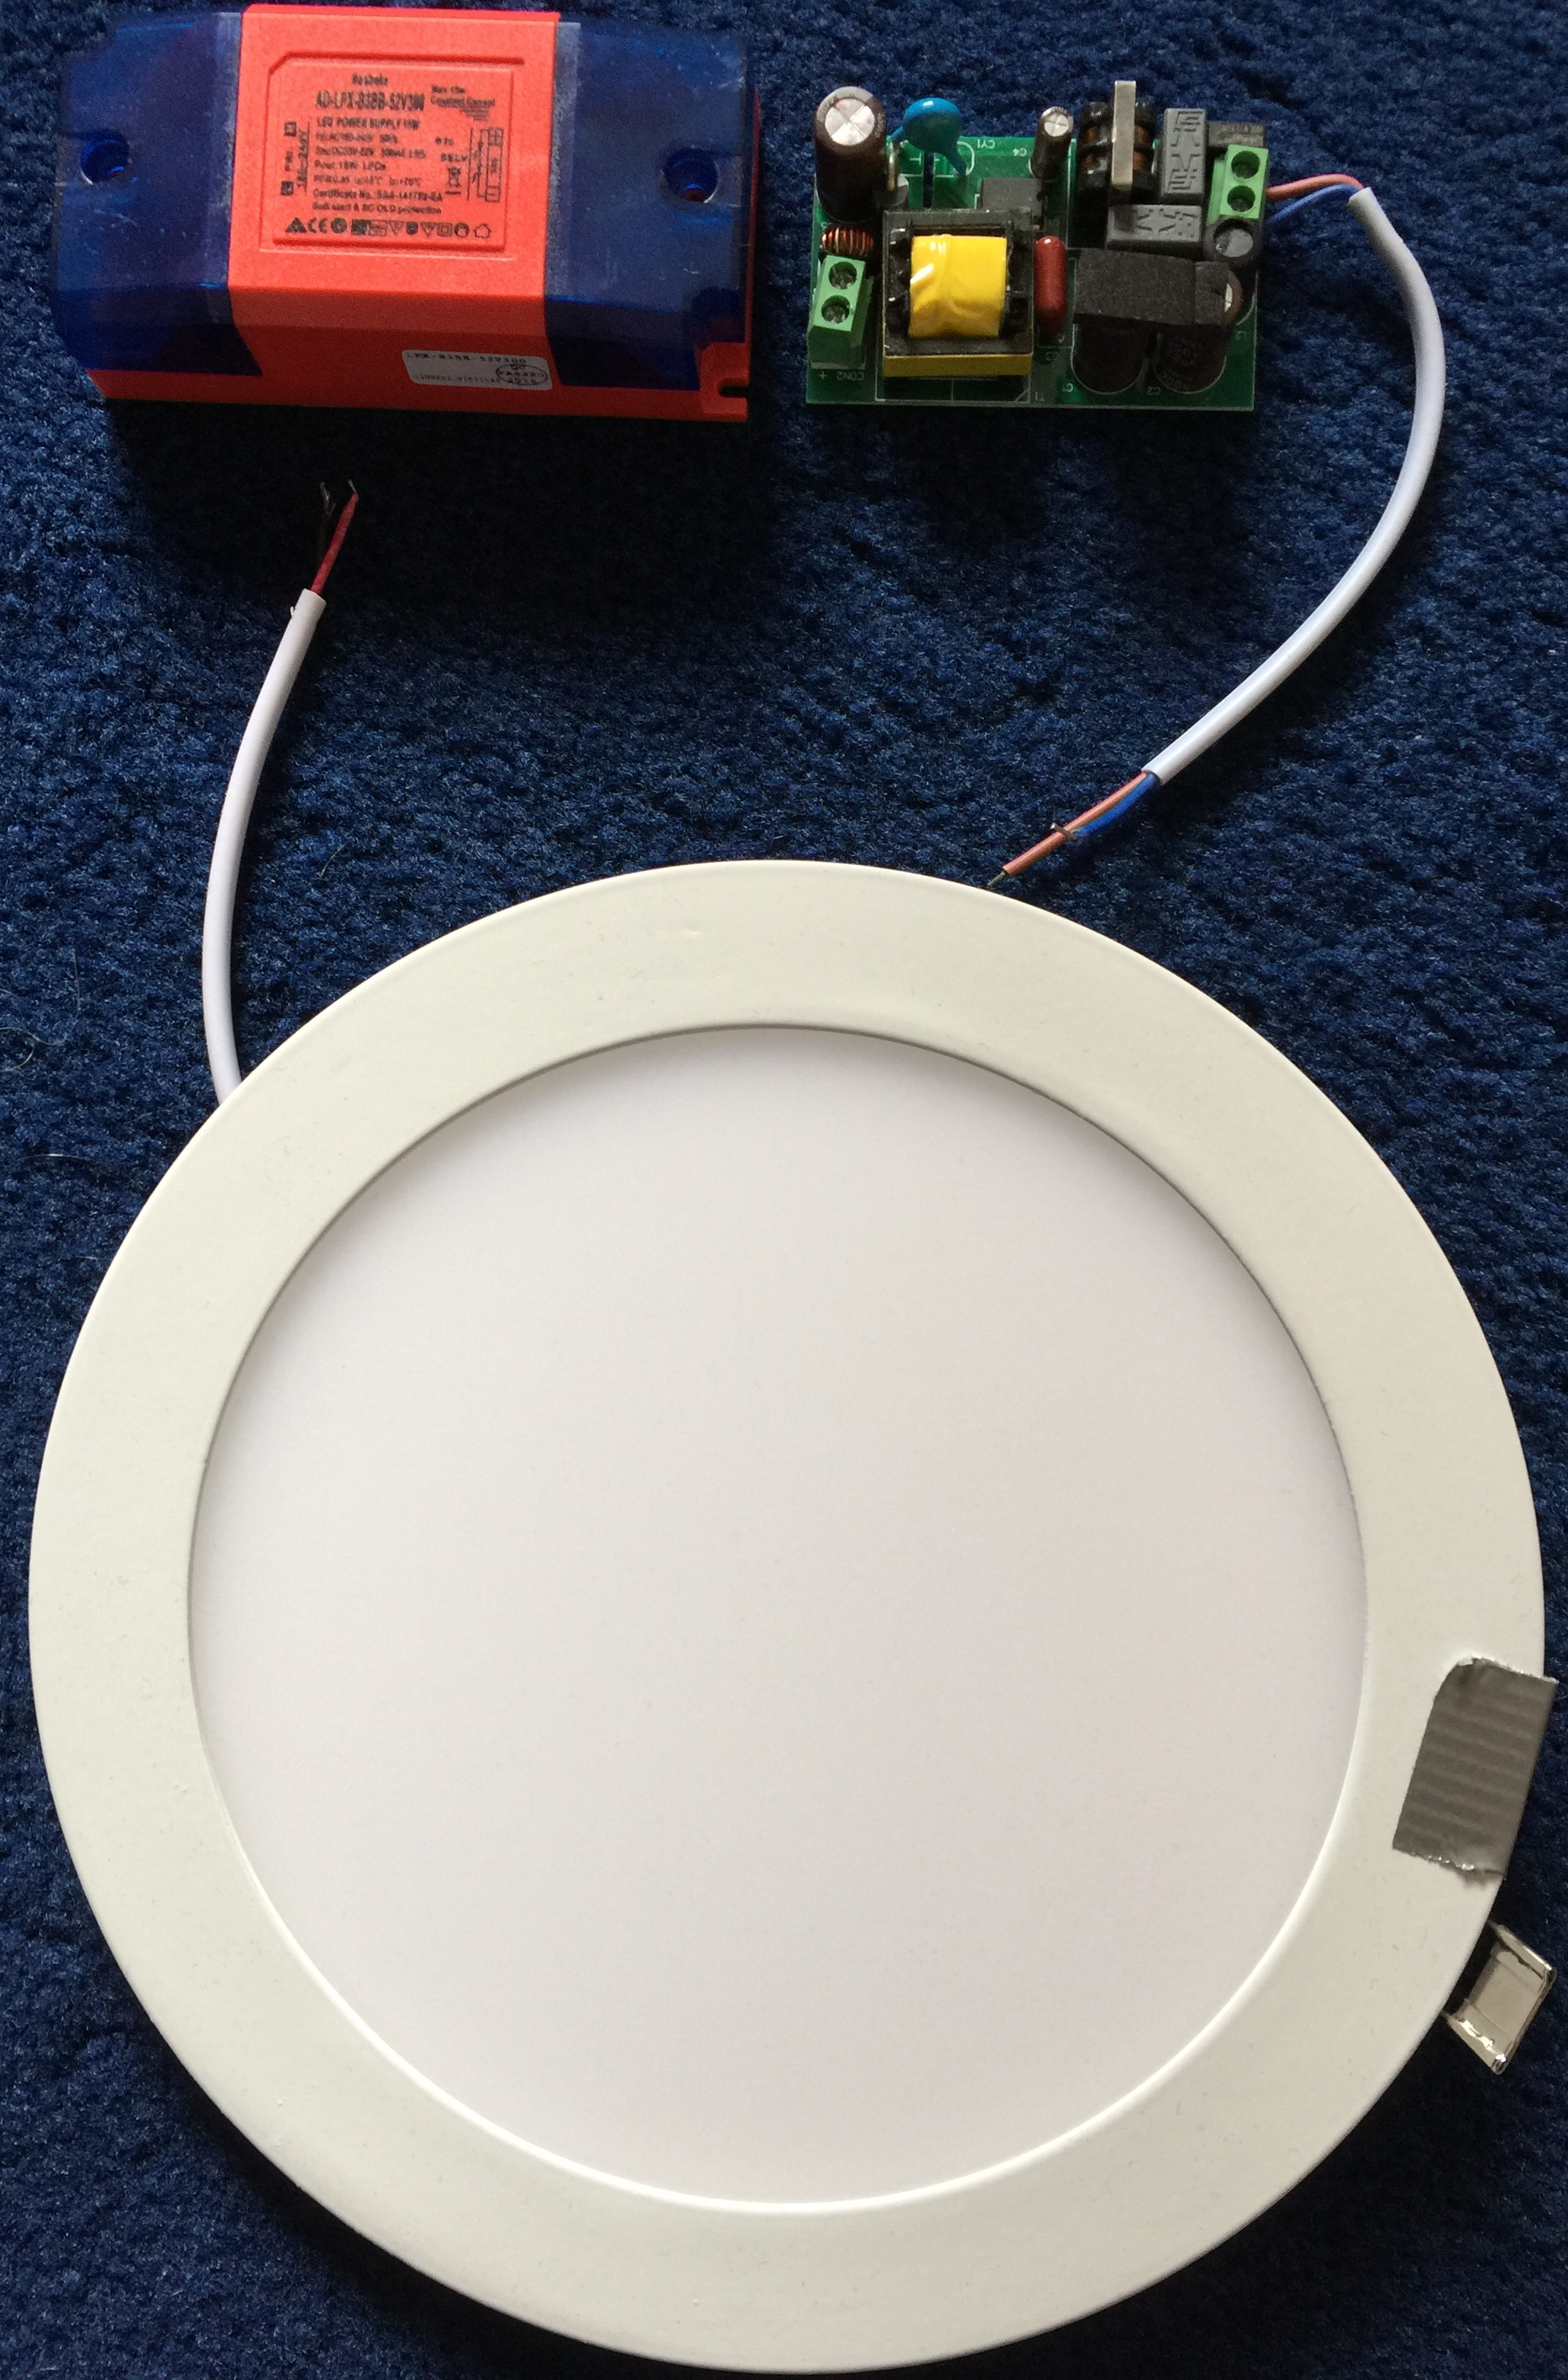
\includegraphics[width=\textwidth]{chapters/hardware-chapters/AC/ac-modulator/smps-led/smps-led-and-smps-picture.jpg}
			\caption{Picture of a commercial LED light fixture with a DC SMPS.}
			\label{fig:ac-smps-led-and-smps-picture}
		\end{minipage}
		\hfill
		\begin{minipage}[b]{0.45\textwidth}
			\centering
			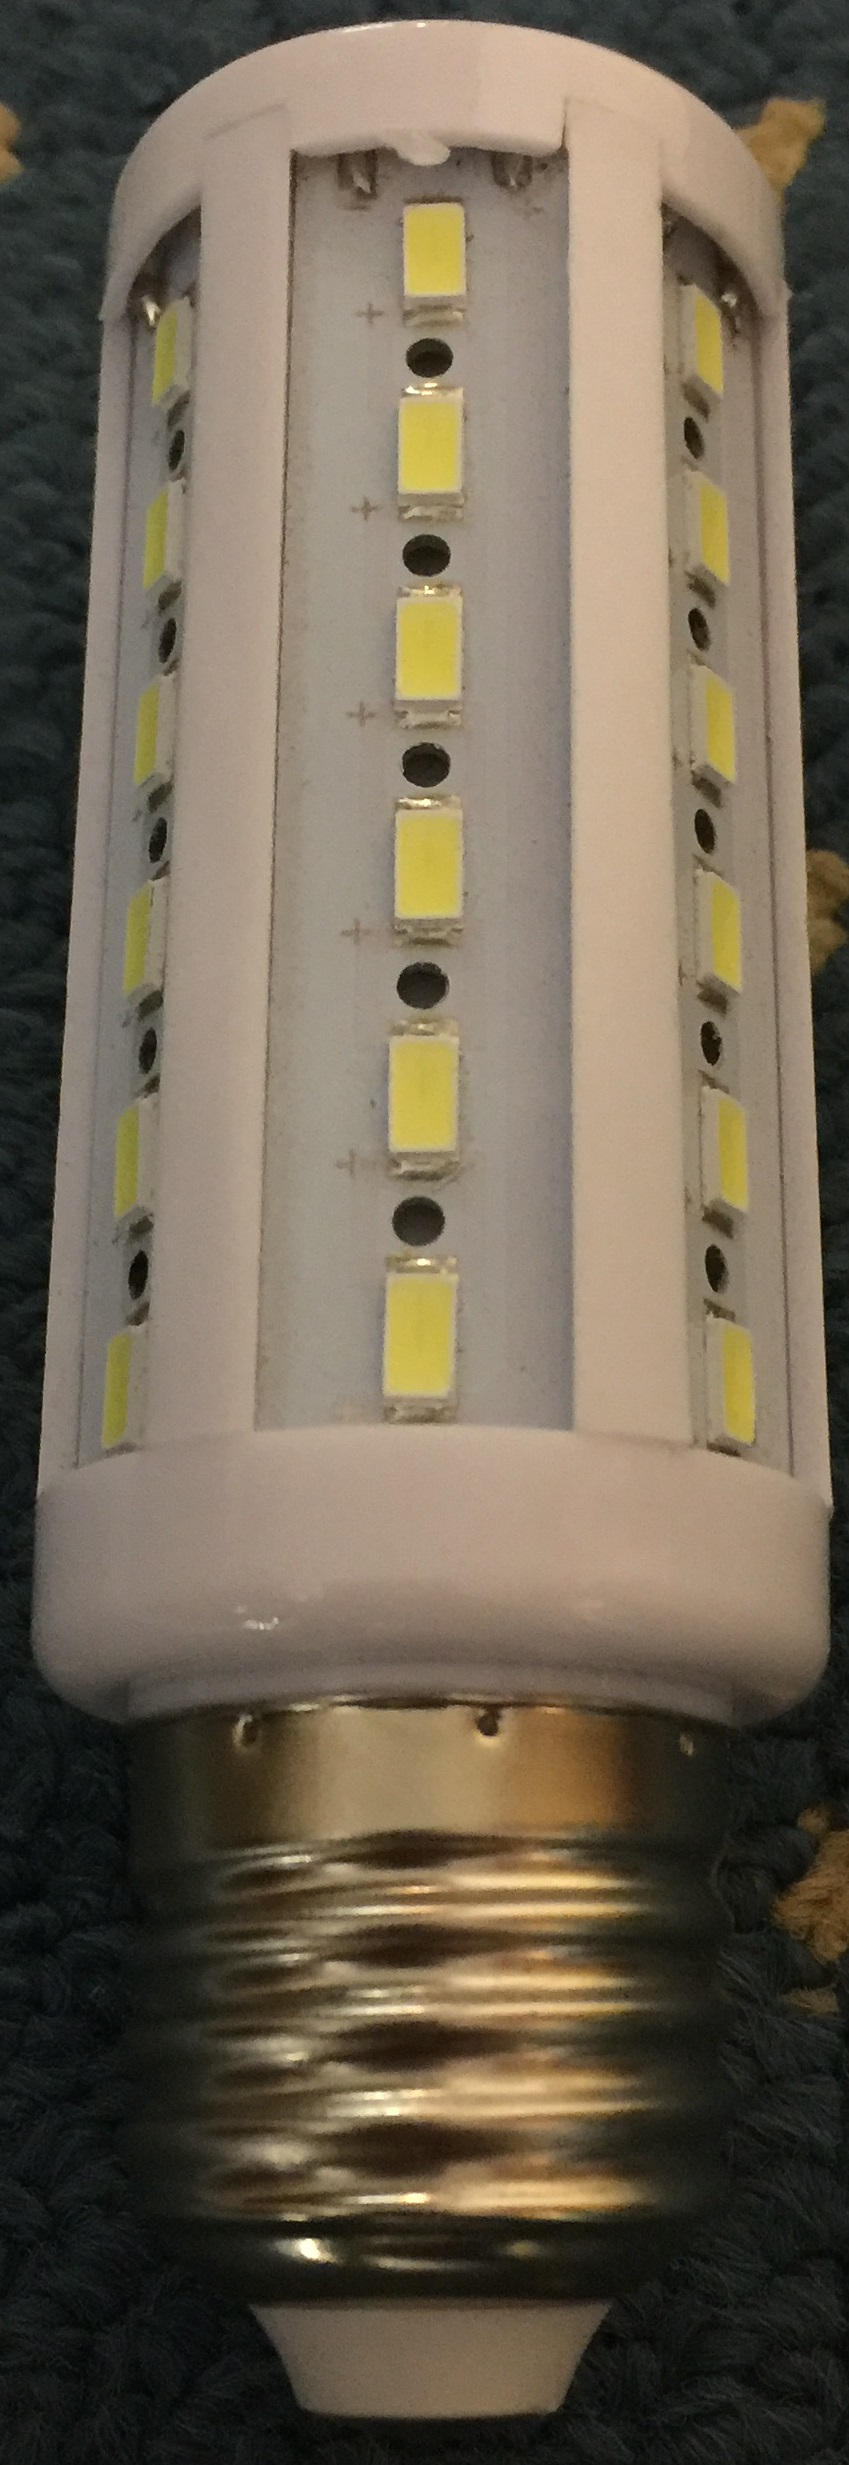
\includegraphics[angle=0,width=0.5\textwidth]{chapters/hardware-chapters/AC/ac-modulator/commercial-230v-ac-led/commercial-ac-led-picture.jpg}
			\caption{Picture of a commercial 230 V AC LED light fixture.}
			\label{fig:ac-commercial-230v-ac-led}
		\end{minipage}
	\end{figure}




% !TeX root = ../../../../../thesis.tex

\subsubsection{230 V AC LED}
\label{subsubsec:ac-230v-led}



There also exists LED lighting fixture which work directly with AC, without having an external SMPS.
An example of such an LED can be seen in \autoref{fig:ac-commercial-230v-ac-led} \cite{commercial-230v-ac-led-aliexpress}.



For this LED it is investigated what the current signature looks like when the LED is constantly on, and when the LED is encoding information.
To measure the current, a 22 ohm resistor is placed in series with the light and the voltage drop over this resistor is measured.
Again, we are only looking at how the current signature behaves, at this point we are not interested in how much current is exactly being drawn.
In order to modulate the LED so that information is encoded in the current, changes had to be made to the internal hardware of the light fixture.
In \autoref{app:commercial-230v-ac-modified-schematic} a schematic can be found, which shows the original circuit and what was modified in order to modulate the LED.
The modifications made, include two transistors to switch the LEDs off and stop the capacitor from charging. 
With these transistors the entire current flow can be stopped and thereby drawing zero current when we want to modulate a zero symbol.
When a `1' symbols needs to be modulated, the transistors are turned on, and the LED behaves in a normal manner.
The transistors are controlled via a micro-controller through an opto-coupler to protect the micro-controller in the development stages.



\begin{figure}[h]
	\centering     %%% not \center
	\subfigure[LED is constantly on. X-axis: 5 ms/div, Y-axis: 1 V/div.]{
		\label{fig:commercial-230v-ac-led-on-annotated}
		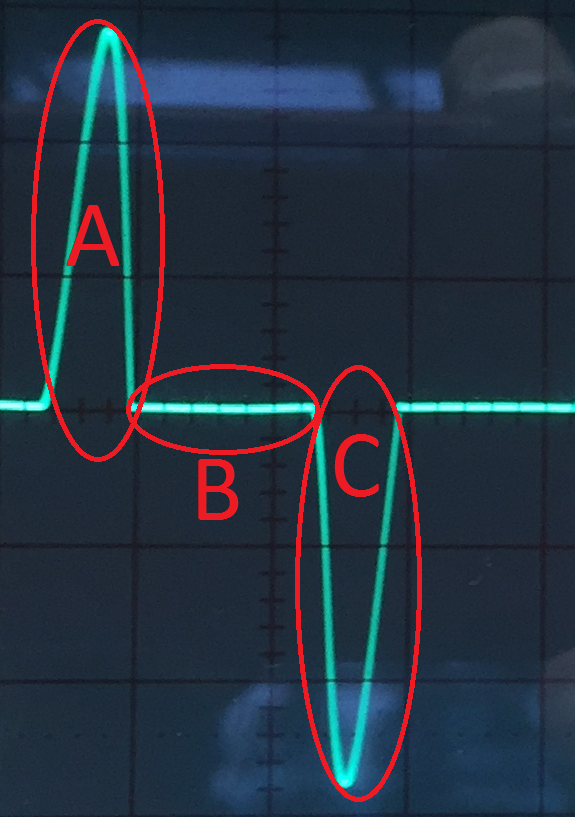
\includegraphics[angle=0,width=0.3\textwidth,keepaspectratio]
		{chapters/hardware-chapters/AC/ac-modulator/commercial-230v-ac-led/commercial-230v-ac-led-on-annotated.png}
	}
	\subfigure[LED is being modulated at 4 kHz. X-axis: 1 ms/div, Y-axis: 5 V/div.]{
		\label{fig:commercial-230v-ac-led-modulating}
		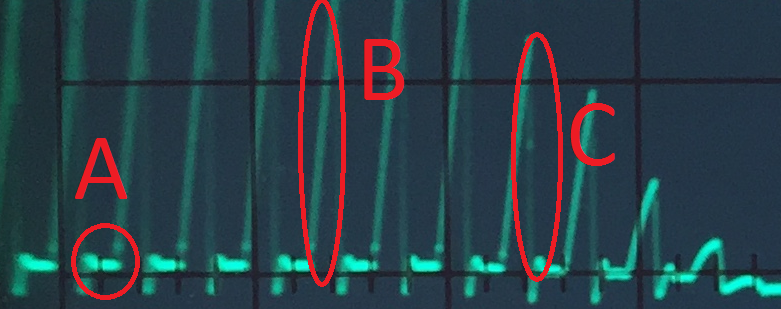
\includegraphics[angle=0,width=0.5\textwidth,keepaspectratio]
		{chapters/hardware-chapters/AC/ac-modulator/commercial-230v-ac-led/commercial-230v-ac-led-modulating-annotated.png}
	}

	\caption{Voltage measured over a 22 ohm series resistor at the primary side, to determine the current signature of a commercial 230 V AC LED.}
\end{figure}



When the LED is off, there is no current draw.
In Figure \ref{fig:commercial-230v-ac-led-on-annotated} the current signature can be seen when the LED is constantly on.
This figure shows 20 ms of the current signal, this is exactly one period of the supplied AC voltage: $t = \frac{1}{f} = \frac{1}{50} = 0.020$ s $= 20$ ms.
Every 20 ms this current draw repeats itself.
In the figure, three regions can be seen: A, B and C.
Each region will now be explained:

\begin{itemize}
	\item In region A, the supplied AC voltage is positive, and so the current that flows is positive.
	As can be seen from the schematic in \autoref{app:commercial-230v-ac-modified-schematic}, all the LEDs are connected in series.
	This means that a certain voltage is required in order for the LEDs to draw current.
	The required voltage is available at the start of region A and is no longer available at the end of region A and the current flow stops.
	The width of the peak is 4 ms.
	The height of the peak indicates how much current is drawn.

	\item The start of region B starts when region A stops.
	The required voltage is no longer available and so the current flow stops and the LED no longer emits light.
	During this region there is no current flow.
	This is a good property: If the LED is off there is no current flow, exactly what we require.

	\item Region C starts when region B stops.
	At this point in time, there is enough voltage available for the LEDs to start drawing current.
	But the voltage that is now available, is not positive as it was in region A, but is negative.
	That is why this peak goes the opposite direction of the peak seen in region A.
	The current that flows is in that case negative, because the voltage is also negative.
	In other aspects this peak has the same properties as those of the peak in region A, it has the same width and height.

\end{itemize}


Only in region A and B, the LED can be used to encode information.
Because in region B, the is no current draw and therefor we cannot modulate information.
The peaks in region A and B are both 4 ms wide.
This means that there is 8 ms of time available for modulation in the 20 ms period, so $\frac{8}{20} = 40$ \% of the time is available for encoding the ID with this LED.
To compare with a DC environment: A DC power supply always supplies a constant voltage, so the LED can always emit light and therefor can always draw current, so 100 \% of the time is available for modulation.
If the ID would have a certain length, it would take time $t$ to modulate this ID in a DC environment and time $2.5 \times t$ with this AC LED. 


Now that the current signature has been investigated when the LED is on, the LED will be now be turned on and off with a frequency of 4 kHz to investigate how the current signature behaves.
In Figure \ref{fig:commercial-230v-ac-led-modulating} the current signature can be seen when the LED is being modulated with a frequency of 4 kHz.
The entire figure takes place inside region A of Figure \ref{fig:commercial-230v-ac-led-on-annotated}.
If this figure would have been showed for region B of Figure \ref{fig:commercial-230v-ac-led-on-annotated}, the amplitudes would have been negative.
Again, there are three regions highlighted:

\begin{itemize}

	\item In region A, the data is being encoded is a `0' and the current draw is also zero.
	As discussed this is a desired property.

	\item Region B shows the transition from the LED being off to the LED being on.
	The current does not go straight up, but instead a slope can be seen.
	This is not a desired property.
	A square wave is desired, this LED is producing a triangular wave.

	\item In region C, the transition from the LED being on to the LED being off can be seen.
	This time the current does go immediately to zero, which is a good property.
	Around region C another issue can be seen. 
	The amplitude of the current becomes lower and lower until region A of Figure \ref{fig:commercial-230v-ac-led-on-annotated} ends.
	This is also not a desirable property, the current should always be some constant value and not decreasing over time.

\end{itemize} 















% !TeX root = ../../../../../thesis.tex

\subsubsection{Custom AC Modulator}






Given the shortcomings of the existing hardware, it was decided to build custom hardware that would behave exactly how it was needed in order to successfully encode information in such a way that the currents could be decoded by a smart-meter.
This means that the current signature should behave very similar to the DC case: For a `0' data bit encoding, the current should be zero and for a `1' data bit encoding, the current should be some constant value.
The transitions between the symbols must be such, that a square wave of current will be created, just like in the DC case. 

\begin{figure}[h]
	\centering
	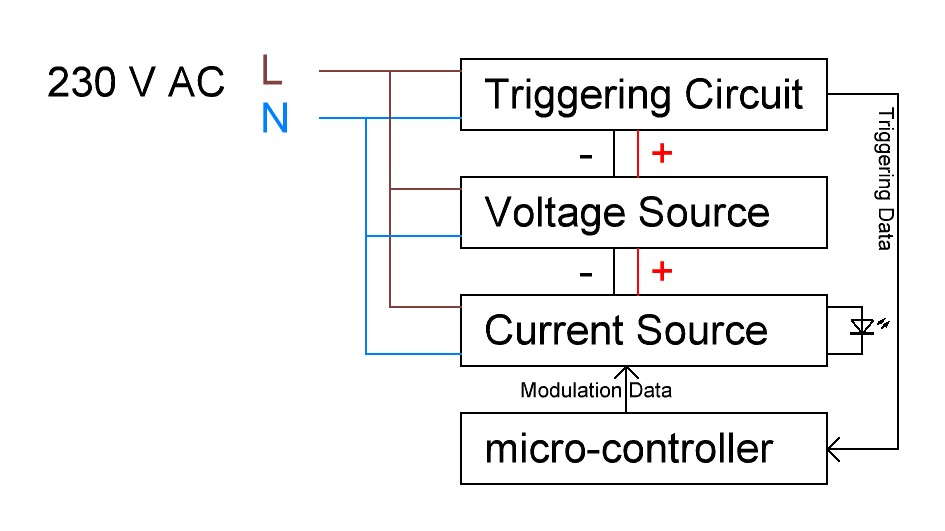
\includegraphics[angle=0,width=0.7\textwidth]{chapters/hardware-chapters/AC/ac-modulator/custom-hardware/ac-modulator-architectural.JPG}
	\caption{Architectural overview of the AC LED modulator.}
	\label{fig:ac-led-modulator-architectural}
\end{figure}

The custom modulator consists of three separate parts: A trigger circuit, a current source and a voltage source.
In \autoref{fig:ac-led-modulator-architectural}, an overview of how these parts are connected to each other can be seen.
The commercial LED that will be used for this solution was already shown \autoref{fig:ac-smps-led-and-smps-picture}, but the SMPS is not used, instead this custom hardware will be powering the LED. 
The entire modulator's schematic can be found in \autoref{app:custom-led-modulator-schematic}.
In the following subsections each part of the hardware of the custom LED modulator will be explained.



% !TeX root = ../../../../../../thesis.tex

\subparagraph{Triggering}

	As discussed before, LEDs need a certain amount of voltage before they draw current.
	That is why Figure \ref{fig:commercial-230v-ac-led-on-annotated} has two separate regions where it draws current, instead of drawing current continuously.
	Given the fact that the ID of the LED cannot be transmitted the entire time, due to the voltage issue, we must somehow give the micro-controller a signal for when the modulation can start and stop.
	If the micro-controller does not have this information, parts of the ID would be encoded when there is no current draw and thus information would be lost, since the encoding of the ID is done with the current draw itself.

	To let the micro-controller know when to start and stop modulating, a triggering circuit is designed.
	This circuit tells the micro-controller when more than a preset voltage is made available by the AC power.
	It also tells the micro-controller when there is less than the preset voltage available.
	In \autoref{fig:triggering-circuit-output-2} the AC voltage can be seen, along with the preset voltage and the corresponding logical output of the triggering circuit.

	%\begin{figure}[h]
	%	\centering
	%	\begin{minipage}[b]{0.39\textwidth}
	%		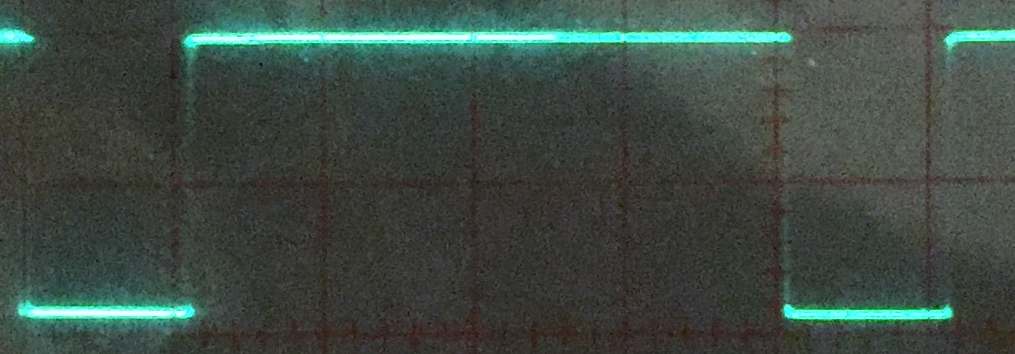
\includegraphics[width=\textwidth]{chapters/hardware-chapters/AC/ac-modulator/custom-hardware/triggering-circuit-output-cropped.png}
	%		\caption{Output from the triggering circuit. Settings: 2 V/div, 2 ms/div.}
	%		\label{fig:triggering-circuit-output}
	%	\end{minipage}
	%	\hfill
	%	\begin{minipage}[b]{0.49\textwidth}
	%		\includegraphics[width=\textwidth]{chapters/hardware-chapters/AC/ac-modulator/custom-hardware/ac-wave-triggering.eps}
	%		\caption{Output form the triggering circuit alongside the incoming AC voltage.}
	%		\label{fig:triggering-circuit-output-2}
	%	\end{minipage}
	%\end{figure}


	\begin{figure}[t]
		\centering
		\begin{minipage}[b]{0.49\textwidth}
			\includegraphics[width=\textwidth]{chapters/hardware-chapters/AC/ac-modulator/custom-hardware/ac-trigger/ac-wave-triggering.eps}
			\caption{Output form the triggering circuit alongside the incoming AC voltage.}
			\label{fig:triggering-circuit-output-2}
		\end{minipage}
		\hfill
		\begin{minipage}[b]{0.49\textwidth}
			\includegraphics[width=\textwidth]{chapters/hardware-chapters/AC/ac-modulator/custom-hardware/ac-trigger/custom-modulator-trigger.JPG}
		    \caption{Triggering circuit to determine when the voltage is sufficiently high enough to start encoding the ID.}
			\label{fig:custom-modulator-trigger}
		\end{minipage}
	\end{figure}

	In \autoref{fig:triggering-circuit-output-2}, the preset voltage is set at 100 V.
	When more than 100 V is available the LED will emit light and start drawing current.
	At that point, around 1 ms in the figure, the triggering circuit will output a logical `1' to the micro-controller, meaning that the encoding of the ID may start.
	When less than 100 V is available, around 9 ms in the figure, the logical output of the circuit becomes `0', indicating to the micro-controller that it is time to stop encoding the ID, else information is lost since the LED is not turning on anymore and therefor no longer draws current.
	The same happens for the negative part of the sine wave, except the preset is now $-100$ V.


	From \autoref{fig:triggering-circuit-output-2} it can be deduced that two times 8 ms is available to encode the ID in a period of 20 ms.
	So $\frac{2 \times 8}{20} = 80$ \% of the time is available for modulation, which is two times more than the 230 V AC LED (Figure \ref{fig:commercial-230v-ac-led-on-annotated}) provided.
	%the solution in \autoref{subsubsec:ac-230v-led}
	To transmit the ID, this solution would be two times faster, but it would still take 25 \% more time than in a DC environment.



	In \autoref{fig:custom-modulator-trigger}, the circuit can be seen which signals the micro-controller when the voltage is more or less than the preset voltage. 
	The voltage preset can be set by using a potentiometer.
	The output of the circuit is electrically isolated from the micro-controller by the means of an optocoupler.
	This is done to protect the micro-controller from the high voltage AC in the development stages.

% !TeX root = ../../../../../../thesis.tex



\subparagraph{Current Source}



	To solve the issue of the non-constant current draw of the other LED solutions, a current source will be used to power the LED.
	The principle is the same as in the DC environment, where also a current source is used.
	In \autoref{fig:custom-modulator-current-source} the schematic for the current source implementation can be seen.
	An optocoupler is used to electrically isolate and protect the micro-controller from the current source, during the development stages.


	\begin{figure}[ht]
		\centering
		\begin{minipage}[b]{0.49\textwidth}
			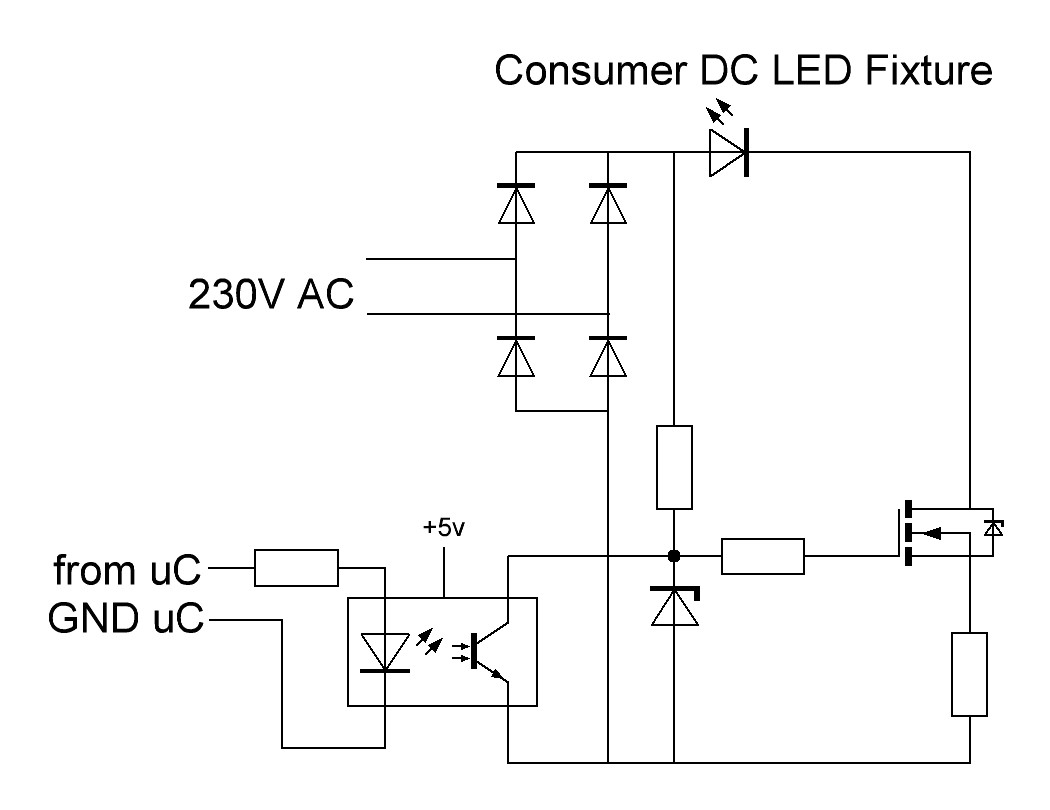
\includegraphics[width=\textwidth]{chapters/hardware-chapters/AC/ac-modulator/custom-hardware/ac-current-source/custom-modulator-current-source.JPG}
			\caption{Current source to power the commercial LED fixture, can be toggled on and off with a microprocessor.}
			\label{fig:custom-modulator-current-source}
		\end{minipage}
		\hfill
		\begin{minipage}[b]{0.49\textwidth}
			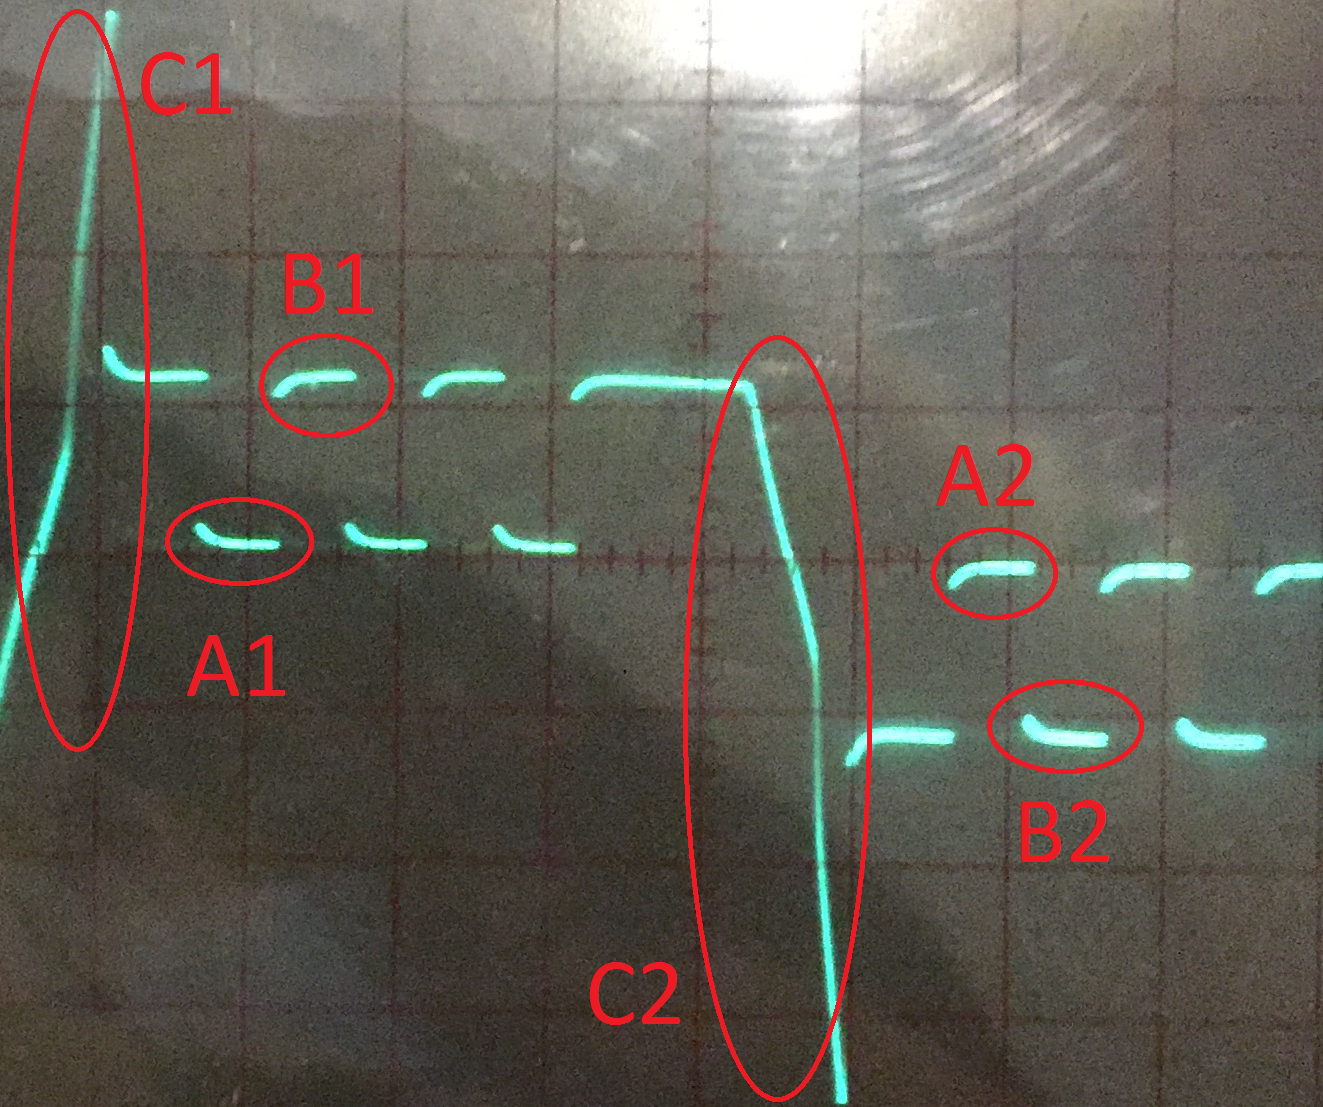
\includegraphics[width=\textwidth]{chapters/hardware-chapters/AC/ac-modulator/custom-hardware/ac-current-source/current-source-measurement-annotated.png}
			\caption{Current that is drawn by the current source. Measured over an 2.8 Ohm resistor. Settings: 200 mV/div, 2 ms/div.}
			\label{fig:current-source-measurement-annotated}
		\end{minipage}
	\end{figure}




	To investigate exactly how the current source implementation performs, a 2.8 Ohm resistor is placed in series with the AC and the current source implementation.
	A micro-controller will toggle the current source on and off via the optocoupler with a frequency of 500 Hz.
	The voltage drop over the series resistor is measured to determine the current draw.
	The result of the current draw can be seen in \autoref{fig:current-source-measurement-annotated}.

	


	In \autoref{fig:current-source-measurement-annotated} six areas are highlighted.
	The regions highlighted with a `1' suffix occur when the supplied AC voltage is positive and the regions with a `2' suffix occur when the AC voltage is negative.
	What happens in these regions will now be explained:


	\begin{itemize}

		\item In region A1 and A2, the LED is turned off because the micro-controller is encoding a `0' and we can see that the current draw is also zero.
		The current draw is zero, independent if the applied AC voltage is positive, in A1, or negative, in A2.


		\item In region B1 and B2, the LED is on, the micro-controller is encoding a `1'. 
		In both regions the current draw remains constant over time, until the LED is turned off.
		But in B1, the current is a positive constant and in B2 the current is a negative constant.
		This is due to the applied AC voltage.
		%In B1 the voltage is positive, so a positive current will flow.
		%And in B2, the voltage is negative, so a negative current will flow.

		\item What happens in regions C1 and C2 is caused by a voltage source, which powers parts of the triggering circuit and the current source.
		What exactly is happening will be explained in the next section, but for now we can assume that it will not affect the encoding of the ID.

	\end{itemize}




	The combination of the trigger circuit and this implementation of a current source allows this solution to detect when to start and stop modulating the LED and it is able to define a specific current draw for the LED.
	This makes mapping the bits `0' and `1' to current levels zero and some constant, easy.
	Which in turn makes detecting the IDs of the LEDs in the smart-meter easy. %which receives an aggregated current, possible.

	






	However, this solution also has a drawback.
	The current source will make sure a constant amount of current will flow through the LEDs.
	The current that flows through the LEDs will cause a voltage difference over the LEDs.
	This is the voltage the LEDs need in order for current to flow, as discussed in the previous sections.
	In the triggering circuit section, it was explained that the LEDs used, require 100 V before the current will flow, see \autoref{fig:triggering-circuit-output-2}.
	This voltage is all the voltage that is needed for these LEDs.
	If less voltage is provided, the LEDs will not emit light.
	But more voltage than necessary will result in power dissipation in some component and will turn into heat.
	Since the applied AC voltage is rated at 230 V RMS, the excessive voltage has to go somewhere.
	This voltage will be dissipated over the current source.
	This means that some energy is being wasted, because there is more voltage provided by the AC than is needed to power the LEDs.



	The other LED solutions discussed above (SMPS LED and 230 V AC LED), solve this problem is two separate manners.
	The SMPS LED, uses a power supply to transform the supplied AC voltage to a certain DC voltage which is exactly what the LEDs need.
	The SMPS has a high efficiency so no power is being wasted, but at the same time this power supply disturbs the encoding of the ID in such a way that the ID is not recognizable anymore.
	The 230 V AC LED uses many LEDs in series and so it requires a very high voltage before the LEDs turn on.
	So only a limited amount of time is used to turn the LEDs on and therefor only a small amount of time is available for modulation of the ID.
	And in the process of encoding the ID, the current is not constant and it does not produce a square wave which makes recognizing the ID difficult.


	The current source implementation, as discussed in this section, solves the encoding problems which the other solutions had.
	But this solution introduces an efficiency problem.
	The priority of this thesis was to create a solution which could recognize which LEDs are on and off by only looking at the aggregated energy consumption.
	The efficiency of this solution has a lower priority.%, which is why this solution was still chosen to develop.
	However, attempts have been made to try and solve the efficiency problem.
	The first attempt involves the use of a transformer and the second attempt uses a capacitor.

	\begin{figure}[b]
		\centering
		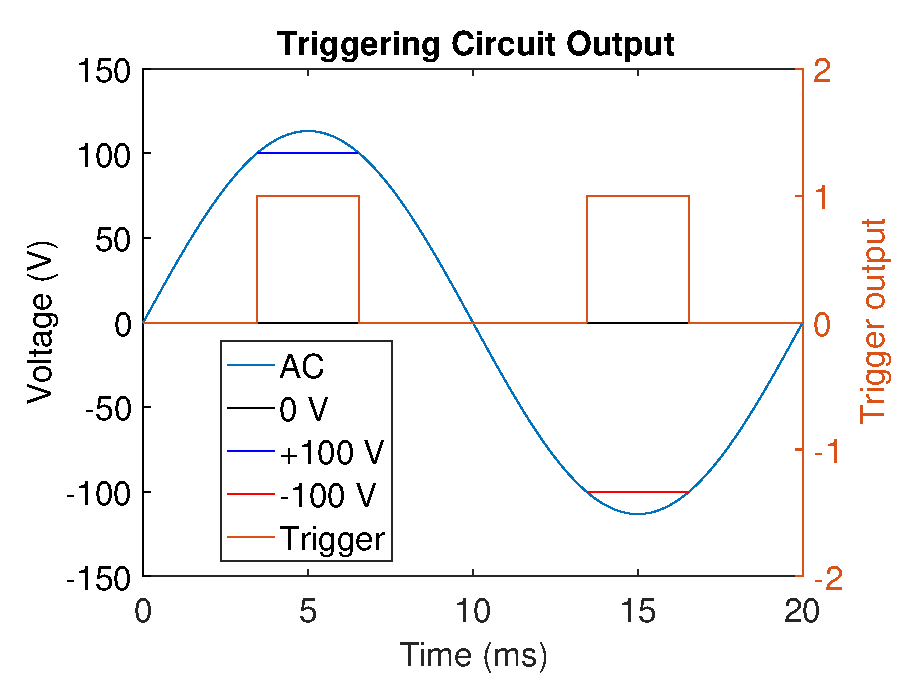
\includegraphics[angle=0,width=0.5\textwidth]{chapters/hardware-chapters/AC/ac-modulator/custom-hardware/ac-current-source/ac-wave-lower-transformed-triggering.eps}
		\caption{Output triggering circuit alongside the output of the AC voltage after a transformer.}
		\label{fig:trigger-output-lower-transformed}
	\end{figure}


	The first attempt uses a transformer to transform the 230 V AC to a lower AC voltage which will solve the efficiency problem.
	The outputted sine wave of the transformer can be seen in \autoref{fig:trigger-output-lower-transformed}.
	The LEDs still need the same amount of voltage: 100V.
	This 100 V threshold can also be seen in \autoref{fig:trigger-output-lower-transformed}.
	The time that is now available for modulation is limited by the use of the transformer, and is 6 ms, which means that only $\frac{6}{20} = 30$ \% of the time is available for modulation.
	Another drawback of using a transformer, is that the distinct current signature that is made using the ID, is distorted by the transformer, as no ideal transformer exists.
	For this reason this solution was abandoned.





	The second attempt showed promising results, however due to time constraints it was not possible to fully investigate this solution. 
	The solution is made up out of two parts: A capacitor and a zero-crossing optotriac.
	The capacitor is placed in series with incoming AC to the rectifying bridge.
	And the optotriac is parallel to this capacitor.
	The schematic can be seen in \autoref{fig:ac-capacitor-triac}.

	\begin{figure}[ht]
		\centering
		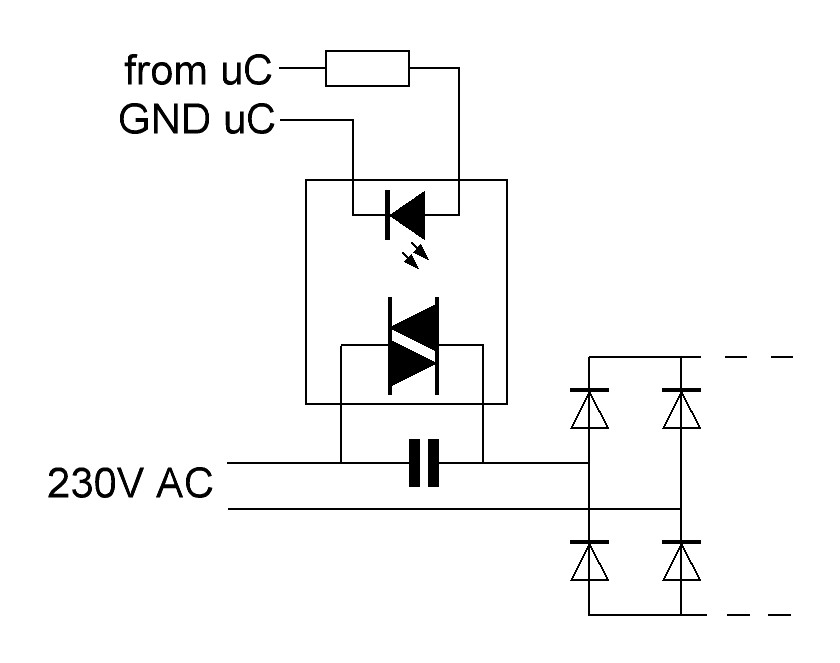
\includegraphics[angle=0,width=0.4\textwidth]{chapters/hardware-chapters/AC/ac-modulator/custom-hardware/ac-current-source/ac-capacitor-triac.JPG}
		\caption{Schematic to show how the capacitor and optotriac are connected.}
		\label{fig:ac-capacitor-triac}
	\end{figure}

	The series capacitor will limit the power that can be consumed by the current source.
	The capacitor is able to do this by phase shifting the current as seen from the voltage.
	In this process the current itself will not be distorted as was the case with using a transformer as discussed above and so the distinct current signature will still be intact.
	The capacitor itself will not dissipate any power and so the efficiency problem can be solved.
	However by limiting the power that the current source can use, there is much less time available to modulate, similar to the solution with the transformer as described above.
	This is were the zero-crossing triac comes in.
	Whenever it is decided to start modulating, the micro-controller activates the triac and then it will short-circuit the capacitor.
	When this happens, effectively the capacitor is no longer connected and it no longer limits the power.
	And so the time available for modulation is restored to the full 80 \%.
	When the transmission of the ID of the LED is finished, the triac is switched off and the capacitor limits the power once again.
	During the transmission of the ID, the current source is dissipating power, but this is only during the transmission of the ID, which is a relative short amount of time.
	Whenever the LED is not transmitting its ID, the capacitor is limiting the power and thus the efficiency issue is solved.
	But due to time constraints it was not possible to fully investigate this solution with the testbed.	




% !TeX root = ../../../../../../thesis.tex


%Both figure side by side to save space...
	%\begin{figure}[!tbp]
	%  \centering
	%  \begin{minipage}[b]{0.48\textwidth}
	%    \includegraphics[width=\textwidth]{chapters/hardware-chapters/custom-modulator-trigger.JPG}
	%    \caption{Triggering circuit to determine when the voltage is sufficiently high enough to start encoding information.}
	%	\label{fig:custom-modulator-trigger}
	%  \end{minipage}
	%  \hfill
	%  \begin{minipage}[b]{0.48\textwidth}
	%    \includegraphics[width=\textwidth]{chapters/hardware-chapters/custom-modulator-voltage-source.JPG}
	%    \caption{Non-disturbing voltage source to power other parts of the circuit.}
	%	\label{fig:custom-modulator-voltage-source}
	%  \end{minipage}
	%\end{figure}



\subparagraph{Non-disturbing Voltage Source}

		
	The two parts of the custom modulator which solve the translation problem of mapping zeros and ones of the ID into the current draw, have now been explained in the prior sections: The triggering circuit and the current source implementation.
	However, as can be seen from the schematics of these parts (\autoref{fig:triggering-circuit-output-2} and \autoref{fig:custom-modulator-current-source}), a 5 Volt voltage source is required to power parts of these circuits.
	In this section it will be explained where this voltage comes from and how it is able to provide this voltage while not distorting the distinct current signature of the ID.


	In the triggering circuit section, it is explained that the LEDs need 100 V before they draw current.
	So every time the voltage is above 100 V the encoding of the ID may begin and whenever the voltage drops below 100 V the encoding stops.
	So whenever the voltage is below 100 V, it does not matter what current is drawn, because no encoding of the ID will take place there.
	Below 100 V is an ideal place to let a circuit create a stable 5 V output to power the triggering circuit and the current source, because it will not distort the encoding of the ID.

	As mentioned before the time that is available for modulation, is 16 ms per period of 20 ms.
	During 16 ms, the voltage is above 100 V and $20 - 16 = 4$ ms is the time that the voltage is below 100 V.
	So in 4 ms per period of 20 ms, it is allowed to draw any current necessary to store the required energy to power the trigger and current source circuits.
	And in the remaining 16 ms per period of 20 ms, this stored energy will be consumed by the triggering circuit and the current source.
	During this 16 ms no current will be drawn to create the stable 5 V output.% as this is already done in the 4 ms window when the voltage is below 100 V.

	To store the energy that will be used later on, a capacitor is used.
	The output of this capacitor goes to a voltage stabilizer IC that will ensure a stable 5 V output.
	A schematic of the solution can be found in \autoref{fig:custom-modulator-voltage-source}.
	When the capacitor is empty, the capacitor is charged by the AC only when the voltage is below 100 V.
	The charging of the capacitor causes a current spike as could already be seen in \autoref{fig:current-source-measurement-annotated}.
	In this figure, regions C1 and C2 clearly show this current spike.
	But since no encoding is done in this region, it will not interfere with the encoding.
	This solution provides a continuous stable 5 V voltage source without distorting the encoding of the ID, since the encoding and the voltage source work in different time sections.

	\begin{figure}[t]
		\centering
		\includegraphics[angle=0,width=0.8\textwidth]{chapters/hardware-chapters/AC/ac-modulator/custom-hardware/ac-voltage-source/custom-modulator-voltage-source.JPG}
		\caption{Non-disturbing voltage source to power other parts of the circuit.}
		\label{fig:custom-modulator-voltage-source}
	\end{figure}
	
















